\begin{frame}{integer representation}
    \begin{itemize}
        \item modern machine represent integers as series of \myemph{bits} (base-2)
        \item why not base-10?
    \end{itemize}
\end{frame}

\begin{frame}{ENIAC: base-10 representation}
\begin{tikzpicture}
\node (eniacPic) {
    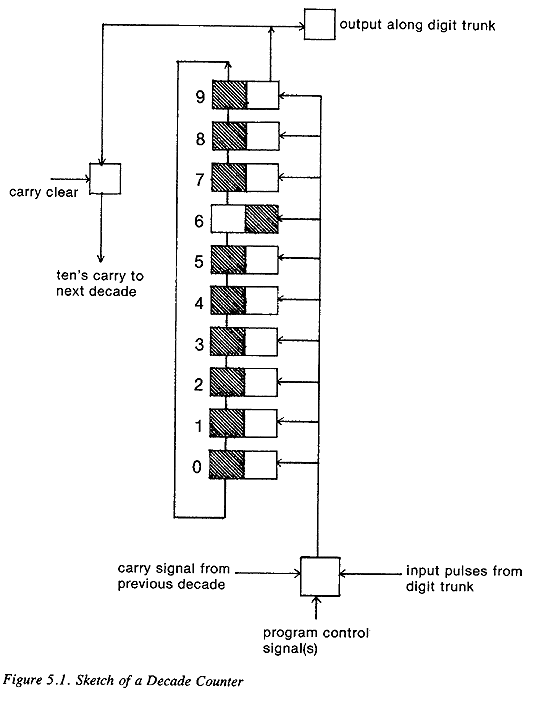
\includegraphics[width=7cm]{Reckoners-fig-05-01}
};
    \node[right=-2cm of eniacPic,align=left] {
        ENIAC: 1946 computer \\
        stored base-10 digits \\
        ~ \\
        ``ring counter'' of ten \\
        electronic switches per digit \\
   };
\end{tikzpicture}
\end{frame}

% FIXME: base-2 switches
